\documentclass{ximera}

\input{preamble.tex}

\author{Gregory Hartman \and Matthew Carr}
\license{Creative Commons 3.0 By-NC}
\acknowledgement{https://github.com/APEXCalculus}

\begin{document}
\begin{exercise}

\outcome{Identify when a limit does not exist.}
\outcome{Calculate limits of piecewise functions.}

\tag{limit} 
\tag{piecewise} 
\tag{trigonometric}
\tag{discontinuous}

  Find 
  \[
  \lim_{x\to \pi/2} f\p{x}
  \begin{prompt}
  = \answer{\text{DNE}}.
  \end{prompt}
  \]
  where
  \[
  f\p{x} = \left\{\begin{array}{cl} \sin\p{x} x & x\leq \pi/2, \\ \cos\p{x} x & x>\pi/2. \end{array}\right.
  \]
    \begin{hint}
     Both pieces of $f\p{x}$, $\sin\p{x} x$, for $x\leq\pi/2$, and $\cos\p{x} x$, for $x>\pi/2$ are continuous for all $x$. However, for the limit $\lim_{x\to\pi/2}f\p{x}$ to exist, both the left-hand and the right-hand limits of $f\p{x}$ at $\pi/2$ must exist and be equal.
    \end{hint}
     \begin{hint}
    	Take a look at the graph of the function
    \begin{center}
     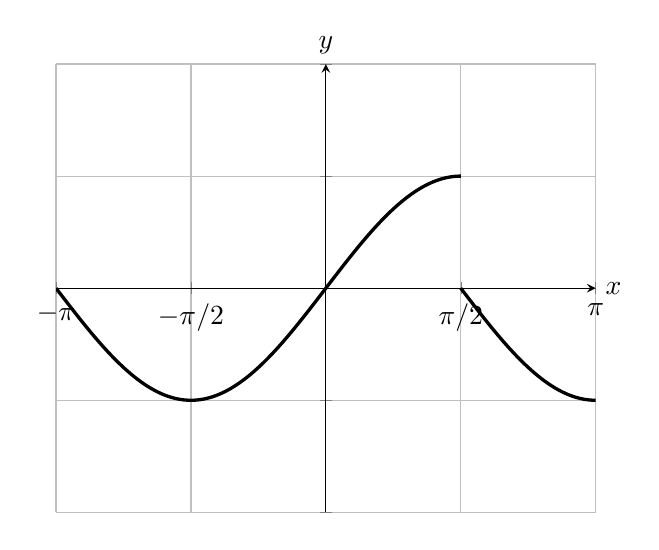
\begin{tikzpicture}
	\begin{axis}
	[ymin=-2,ymax=2, axis lines=center,xlabel=$x$,ylabel=$y$,every axis y 
	label/.style={at=(current axis.above origin),anchor=south},every axis x label/.style={at=(current axis.right of origin),anchor=west},
	domain=-pi:pi,
	yticklabels={},
	xtick={-3.141592653589793,-1.570796326794897,0,1.570796326794897,3.141592653589793},
	xticklabels={$-\pi$,$-{\pi}/{2}$,$0$,${\pi}/{2}$,$\pi$},
	ymajorgrids=true,
	grid = major
	]
	\addplot[domain=-pi:pi/2,very thick,smooth,samples=1000]
	{sin(deg(\x))};
	\addplot[domain=pi/2:pi,very thick,smooth,samples=1000]
	{cos(deg(\x))};
	\end{axis}
       \end{tikzpicture}      
      \end{center} 
    \end{hint}
    \begin{hint}
     Evaluating $\lim_{x\to{\pi/2}^{+}}f\p{x}$ we see that it is equal to $\cos\p{x} \pi/2=0$. This follows because, for $x>\pi/2$, we are on the piece of $f\p{x}$ given by $\cos\p{x} x$ and the limit $\lim_{x\to{\pi/2}}\cos\p{x} x=0$, certainly. On the other hand, evaluating $\lim_{x\to{\pi/2}^{-}}f\p{x}$ we see it is equal to $\sin\p{x} \pi/2=1$. This follows because, for $x\leq\pi/2$, we are on the piece of $f\p{x}$ given by $\sin\p{x} x$ and the limit $\lim_{x\to\pi/2}\sin\p{x} x=1$, certainly. These are not equal, so $\lim_{x\to\pi/2}f\p{x}$ does not exist.
    \end{hint}
\end{exercise}

\end{document}